\documentclass[12pt]{article}

\usepackage{fullpage}
\usepackage{multicol,multirow}
\usepackage{tabularx}
\usepackage{ulem}
\usepackage[utf8]{inputenc}
\usepackage[russian]{babel}
\usepackage{hyperref}
\usepackage{amsmath}
\usepackage{listings}
\usepackage{graphicx}
\usepackage{color}
\usepackage{amsfonts}

\begin{document}

\begin{titlepage}
\begin{center}

\bfseries{\Large Московский авиационный институт\\ (национальный исследовательский университет)}

\vspace{48pt}


{\large Факультет информационных технологий и прикладной математики}

\vspace{36pt}


{\large Кафедра вычислительной математики и программирования}

\vspace{48pt}


\vspace{12pt}

Курсовой проект по курсу Численные методы\\
по теме: "Аппроксимация функций с использованием вейвлет-анализа"


\end{center}

\vspace{100pt}

\vfill

\begin{flushleft}
Студентка: Е.\,Н. Безлуцкая \\
Преподаватель: Д.\,Л. Ревизников \\
Группа: М8О-307Б\\
Дата:\\
Оценка:\\
Подпись:\\
\end{flushleft}

\vspace{12pt}


\begin{center}
\bfseries Москва, \the\year
\end{center}
\end{titlepage}

\pagebreak

\section*{Постановка задачи}

Взять некоторую периодическую функцию и аппроксимировать с помощью дискретного вейвлет-преобразования(ДВП). Получить, используя прямое ДВП, коэффициенты аппроксимации и коэффициенты детализации. Затем провести обратное преобразование, получить исходную функцию.
Обнаружить локальные характеристики функции.

\section*{Описание}
\subsection*{Введение}
Известно, что преобразование Фурье обладает существенным недостатком, а именно неспособностью отслеживать частотно-временные характеристики сигнала с течением времени. Чтобы этот недостаток устранить, в качестве анализирующей функции нужно выбирать не гармоническую, растянутую по всей числовой оси, а некую функцию, локализованную на этой оси. Так, вейвлет-преобразования  основаны на разложении по малым волнам,
называемым вейвлетами, изменяющейся частоты и ограниченным во времени (в пространстве).

\subsection*{Кратномасштабное разложение}
Функцию (сигнал) $f(x)$ часто проще анализировать, если представить ее в виде
линейной комбинации функций из некоторой системы функций разложения $\{\phi(x)\}$
\[
f(x) = \sum_k \alpha_k \phi_k(x), \tag{1}
\]
где $k$ -- конечное или бесконечное множество целых значений, вещественные числа $\alpha_k$ -- \textit{коэффициенты разложения}, $\phi_k$ принимают вещественные значения и называются \textit{функциями разложения}. Если разложение единственно, то функции $\phi_k(x)$ называются базисными функциями, а все множество функций разложения $\{\phi(x)\}$ называется базисом в том классе функций, которые могут быть представлены таким образом. Представимые в виде (1) функции образуют \textit{пространство функций}
$$V = \overline{\underset{k}{Span}\{\phi(x)\}}$$
,которое называется замыканием линейной оболочки функций $\{\phi(x)\}$ или пространством, натянутым на систему
функций $\{\phi(x)\}$.\\
\\
Рассмотрим систему функций разложения, которая состоит из целочисленных сдвигов и двоичных изменений масштаба некоторой заданной вещественной квадратичноинтегрируемой функции $\phi(x)$. Таким образом, мы рассматриваем систему функций $\{\phi_{j,k}(x)\}$ вида
\[
\phi_{j,k} = 2^{j/2}\phi(2^j x - k), \tag{2}
\]
где $j,k \in \mathbb{Z}$ и $\phi(x) \in L^2(\mathbb{R})$. Здесь $k$ определяет положение функции $\phi_{j,k}(x)$ на оси $x$, индекс $j$ — ширину функции $\phi_{j,k}(x)$ вдоль оси x, а множитель $ 2^{j/2}$ регулирует высоту (амплитуду) функции. Функция $\phi(x)$ называется \textit{масштабирующей функцией}.\\
\\
Если мы ограничимся рассмотрением какого-нибудь одного фиксированного значения $j$ в (2), скажем, $j = j_0$, то получаемая в результате система функций разложения $\phi_{j_0,k}$ будет подмножеством всей системы функций $\phi_{j,k}$. Тогда определим подпространство для $L^2(\mathbb{R})$ выражением
\[
V_{j_0} = \overline{\underset{k}{Span}\{\phi(x)\}}. \tag{3}
\]
Если $f(x) \in V_{j_0}$, то она может быть заисана в виде
\[
f(x) = \sum_k \alpha_k \phi_{j_0,k}(x), \tag{4}
\]
Часто используется, например, масштабирующая функция Хаара:\\
\[
\phi(x) = 
\begin{cases}
1,    & 0 \leq x < 1\\
0,    & \text{в остальных случаях.}\\
\end{cases}
\tag{5}
\]
Если задана масштабирующая функция, удовлетворяющая КМА-условиям:
\begin{enumerate}
\item Масштабирующая функция и ее целые сдвиги ортогональны
\item Подпространства, натянутые на систему масштабирующих
функций при низком разрешении (в мелком масштабе), содержатся в подпространствах, натянутых на систему масштабирующих функций при более высоком разрешении (в более крупном масштабе)
\item Единственной функцией, принадлежащей одновременно всем
подпространствам $V_j$ , является функция $f(x) = 0$
\item Любая функция может быть представлена с произвольной
точностью
\end{enumerate}
, то можно определить такую \textit{вейвлет-функцию} $\psi(x)$(материнский вейвлет), что система функций, состоящих из целых сдвигов и двоичных изменений масштаба функции $\psi(x)$, порождает разность между двумя смежными КМА-подпространствами $V_j$ и $V_{j+1}$. Определим систему вейвлетов
\[
\psi_{j,k}(x) = 2^{j/2}\psi(2^j x - k), \tag{6}
\]
и каждое из пространств $W_j$ оказывается натянутым на подсистему
$\{\psi_{j,k}(x)\}$ при $k \in \mathbb{Z}$. Как и ранее, мы записываем
\[
W_j = \overline{\underset{k}{Span}\{\psi_{j,k}(x)\}}. \tag{7}
\]
и если $f(x) \in W_j$, то
\[
f(x) = \sum_k \alpha_k \psi_{j,k}(x), \tag{8}
\]
Подпространства, порождаемые масштабирующей функцией
и вейвлет-функцией, связаны между собой соотношением
\[
V_{j+1} = V_j + W_j, \tag{9}
\]
Часто используется, например, вейвлет-функция Хаара:\\
\[
\psi(x) = 
\begin{cases}
1,    & 0 \leq x < 0.5;\\
-1,   & 0.5 \leq x < 1;\\
0,    & \text{в остальных случаях.}\\
\end{cases}
\tag{10}
\]

\subsection*{Дискретное вейвлет-преобразование}
Подобно разложению в ряд Фурье разложение в вейвлет-ряд ставит в соответствие функции непрерывного аргумента некоторую последовательность коэффициентов. В том случае, когда подлежащая разложению функция является дискретной (т. е. последовательностью чисел), получаемая последовательность коэффициентов называется \textit{дискретным вейвлет-преобразованием} функции f(x). Например, если $f(n) = f(x_0 + n\Delta x)$ для некоторых значений $x_0$, $\Delta x$ и $n = 0, 1, 2, ..., M - 1$ коэффициенты разложения
$f(x)$ в вейвлет-ряд становятся коэффициентами \textit{прямого} ДВП последовательности $f(n)$:
\[
W_\phi(j_0,k) = \dfrac{1}{\sqrt{M}} \sum_n f(n) \phi_{j_0,k}(n),
\tag{11}
\]

\[
W_\psi(j,k) = \dfrac{1}{\sqrt{M}} \sum_n f(n) \psi_{j,k}(n) \quad \text{для} \quad j \geq j_0.
\tag{12}
\]
\\
В формулах выше\\
$\phi_{j_0,k}(n)$ и $\psi_{j,k}(n)$ -- дискретные версии базисных функций $\phi_{j_0,k}(x)$ и $\psi_{j,k}(x)$\\
$W_\phi(j_0,k)$ -- коэффициенты приближения\\
$W_\psi(j,k)$ -- коэффициенты деталей\\
\\
Дополнением к прямому будет обратное ДВП вида\\
\[
f(n) = \dfrac{1}{\sqrt{M}} \sum_n W_\phi(j_0,k) \phi_{j_0,k}(n) + \dfrac{1}{\sqrt{M}} \sum_{j = j_0}^{+\infty} \sum_k W_\psi(j,k) \psi_{j,k}(n).
\tag{13}
\]
Обычно полагают $j_0 = 0$ и выбирают число $M$ так, чтобы оно было степенью двойки (т.е. $M = 2^J$); при этом суммирование в уравнениях (11)—(13) производится по значениям $n = 0, 1, 2, ..., M - 1$, $j = 0, 1, 2, ..., J - 1$ и $k = 0, 1, 2,
..., 2^J - 1$. Для системы Хаара дискретные аналоги масштабирующих функций и вейвлет-функций (т.е. базисных функций), участвующих в преобразовании, соответствуют строкам $M \times M$ матрицы преобразования Хаара \textbf{H}.\\
\\
Матрица \textbf{H} состоит из из базисных функций Хаара $h_k(z)$. Эти функции определены на непрерывном замкнутом интервале $z \in [0, 1]$ при $k = 0,1,2,...,N - 1$, где $N = 2^n$. Чтобы получить \textbf{H}, зададим целое $k$ такое, что $k = 2^p + q - 1$,\\
\\
где $0 \leq p \leq n - 1$,\\
\\
$
q = 
\begin{cases}
0, 1                & \text{при } l = 0\\
1 \leq q \leq 2^p   & \text{при } l \neq 0\\
\end{cases}
$\\
\\
Тогда \textit{базисные функции Хаара} будут
$$h_0(z) = h_{00}(z) = \dfrac{1}{\sqrt{N}}, \quad z \in [0,1]$$
и \[
h_k(z) = h_{pq}(z) = \dfrac{2^{p/2}}{\sqrt{N}}
\begin{cases}
1    & \text{при } (q - 1) / 2^p \leq z \leq (q - 0.5) / 2^p\\
-1   & \text{при } (q - 0.5) / 2^p \leq z \leq q / 2^p\\
0    & \text{в остальных случаях, } z \in [0,1]\\
\end{cases}
\]
\\
Само преобразование состоит из M коэффициентов, минимальный масштаб равен нулю, а максимальный равен $J - 1$.

\subsection*{Быстрое вейвлет-преобразование}

Быстрое вейвлет-преобразование (БВП) представляет собой эффективный метод реализации вычислений дискретного вейвлет-преобразования (ДВП), который использует взаимосвязь между коэффициентами ДВП соседних масштабов. Метод БВП называют также иерархическим алгоритмом Малла.\\
\\
ДВП сигнала $x$ получают применением набора фильтров. Сначала сигнал пропускается через низкочастотный (low-pass) фильтр. Одновременно сигнал раскладывается с помощью высокочастотного (high-pass) фильтра. В результате получаются детализирующие коэффициенты (после ВЧ-фильтра) и коэффициенты аппроксимации (после НЧ-фильтра).\\
\\
Это разложение можно повторить несколько раз для дальнейшего увеличения частотного разрешения с дальнейшим прореживанием коэффициентов после НЧ и ВЧ-фильтрации. Это можно представить в виде двоичного дерева, где листья и узлы соответствуют пространствам с различной частотно-временной локализацией. Это дерево представляет структуру банка (гребёнки) фильтров.\\
\begin{figure}[h!]
  \caption{Двухступенчатый или двухмасштабный БВП-банк анализа и его свойства в отношении разделения частот}
  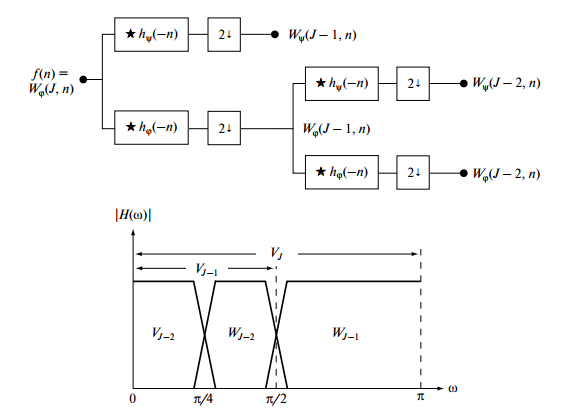
\includegraphics[scale=0.7]{images/1-1.png}
\end{figure}
\newpage
\section*{Результаты}

\subsection*{Прямое ДВП}
В качестве сигнала используется таблично заданная периодическая функция.\\
\\
Для начала возьмем функцию со стационарным частотным спектром $f(x) = sin(2x)$ с масштабом $J = 4$, тогда число значений функции $M = 2^J = 16$\\

\newpage

\textbf{Разложение(уровень1)}\\
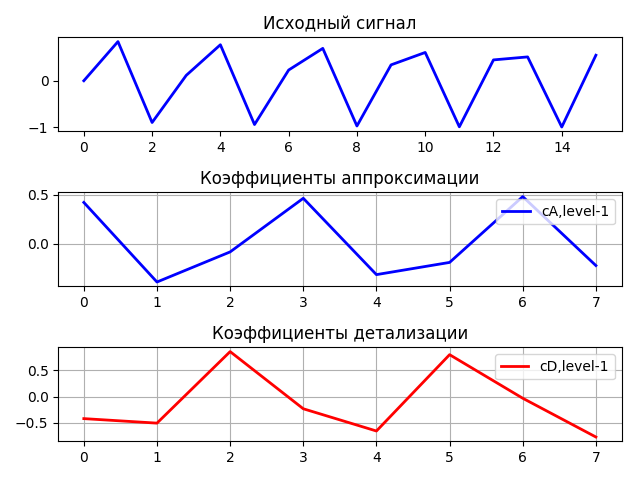
\includegraphics[scale=0.7]{images/2-1.png}\\

\textbf{Разложение(уровень2)}\\
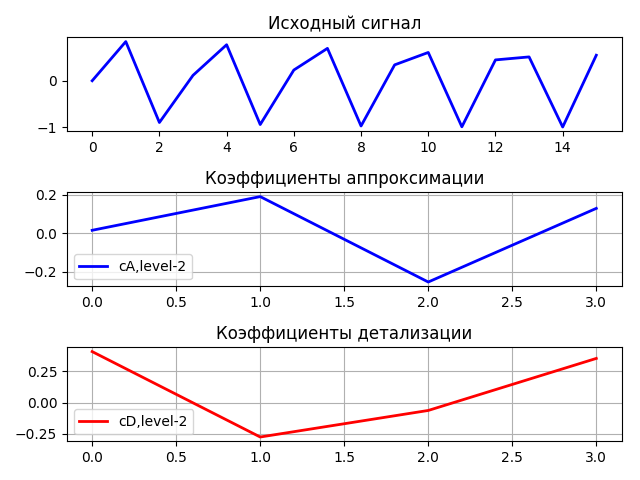
\includegraphics[scale=0.7]{images/2-2.png}\\
\\
Дальнейшее разложение до максимального уровня(4) не имеет смысла, так как малое количество коэффициентов нам не даст никакой интересной информации. Для изучения особенностей вейвлет-преобразования нужно взять сигнал с нестационарным частотным спектром. Например, где, начиная с определенного x, частота функции начинается меняться. В данном примере для наглядности возьмем масштаб больше -- $J = 7$. Возьмем в диапазоне x от 0 до 20 сигнал:\\
\\
$
f(x) = 
\begin{cases}
cos(x) + sin(2x) & \text{, при } x \leq 10\\
cos(x) + sin(6x) & \text{, иначе. }\\
\end{cases}
$\\
\\
\textbf{Разложение(уровень1)}\\
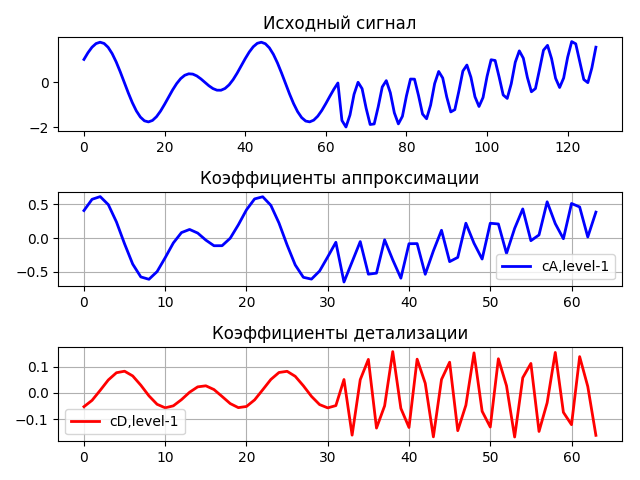
\includegraphics[scale=0.7]{images/3-1.png}\\

\textbf{Разложение(уровень2)}\\
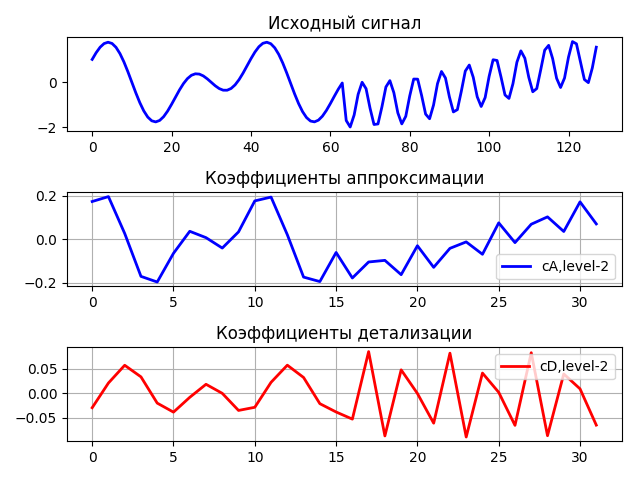
\includegraphics[scale=0.7]{images/3-2.png}\\

\textbf{Разложение(уровень3)}\\
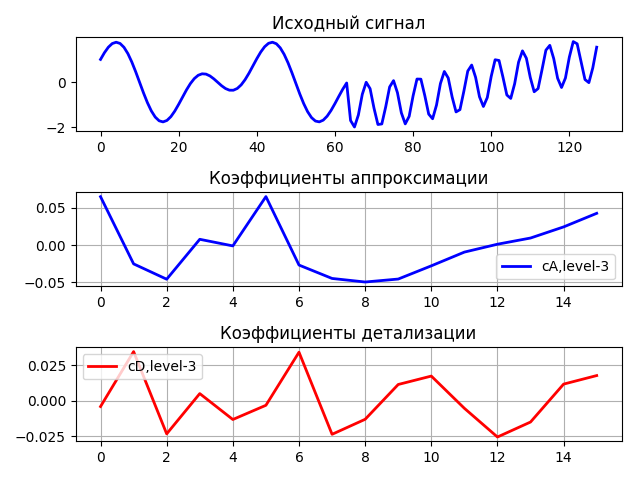
\includegraphics[scale=0.7]{images/3-3.png}\\
\\
На первых уровнях разложения видно, что ДВП хорошо <<отлавливает>>  спектральные характеристики.  Это позволяет нам легко определить, в какой части сигнала произошло изменение частоты спектра.\\
\\
В следующем примере будем использовать сигнал с динамическим частотным спектром, который со временем увеличивается.\\
\\
$
f(x) = sin(x^2)
$
\newpage
\textbf{Разложение(уровень1)}\\
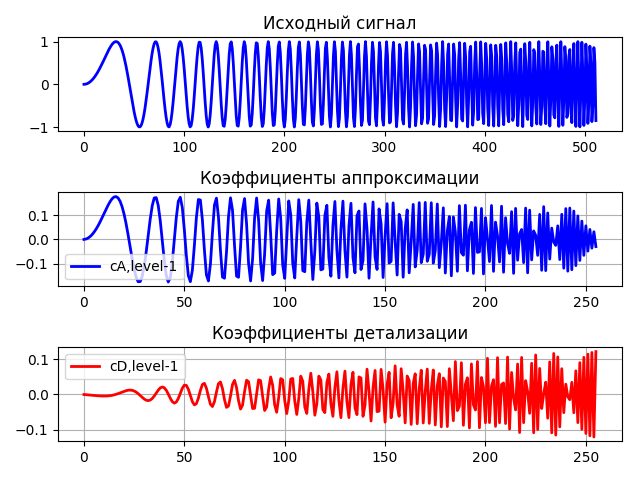
\includegraphics[scale=0.7]{images/4-1.png}\\

\textbf{Разложение(уровень5)}\\
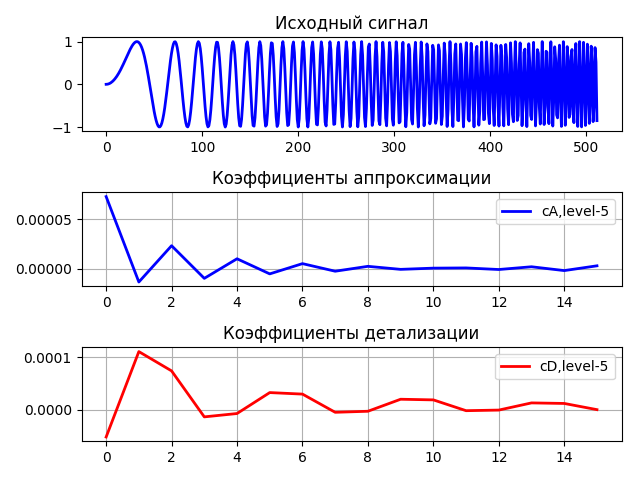
\includegraphics[scale=0.7]{images/4-2.png}\\

Можно заметить, что начиная с определеленного уровня, функция начинает <<сглаживаться>> в области высоких частот. Это подводит нас к тому, что с помощью вейвлет-преобразования можно удалять из сигнала шум.
\newpage

\textbf{Разложение(уровень1)}\\
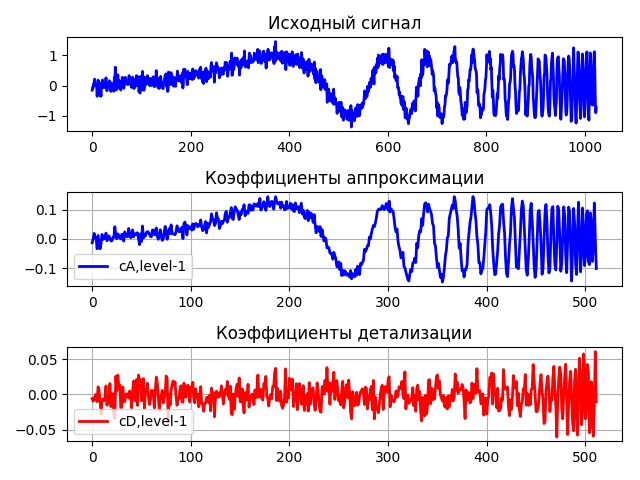
\includegraphics[scale=0.7]{images/5-1.png}\\

\textbf{Разложение(уровень3)}\\
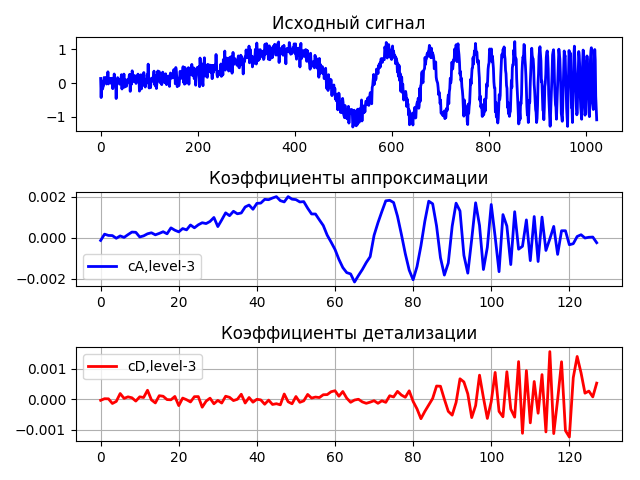
\includegraphics[scale=0.7]{images/5-2.png}\\
\newpage

\textbf{Разложение(уровень4)}\\
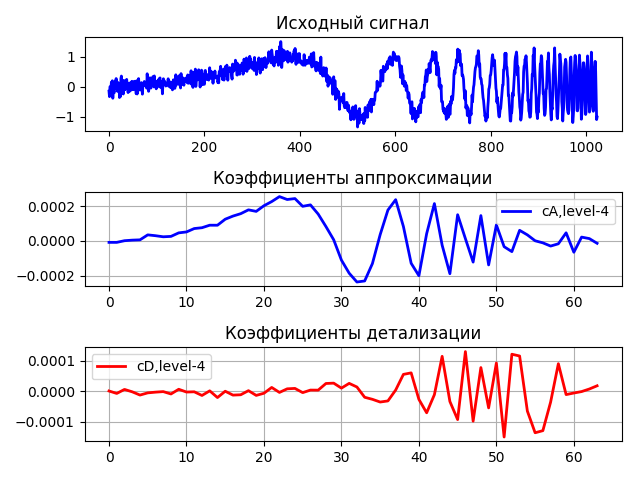
\includegraphics[scale=0.7]{images/5-3.png}\\
\\
При масштабе, равном десяти, уже на уровне три-четыре заметно удаление шума.

\subsection*{Обратное ДВП}

Для демонстрации обратного ДВП возьмем простой короткий сигнал ($J = 3$) и получим исходную функцию из коэффициентов разного уровня:\\
\\
\begin{lstlisting}
Signal: [1, 2, 3, 4, 5, 6, 7, 8]
Coefficients in level = 1:  [array([  2.121,   4.95 ,   7.778,  10.607]), 
array([-0.707, -0.707, -0.707, -0.707])]
Signal by coefficients:  [ 1.  2.  3.  4.  5.  6.  7.  8.]

Coefficients in level = 2:  [array([  5.,  13.]), array([-2., -2.]), 
array([-0.707, -0.707, -0.707, -0.707])]
Signal by coefficients:  [ 1.  2.  3.  4.  5.  6.  7.  8.]

Coefficients in level = 3:  [array([ 12.728]), array([-5.657]),
 array([-2., -2.]), array([-0.707, -0.707, -0.707, -0.707])]
Signal by coefficients:  [ 1.  2.  3.  4.  5.  6.  7.  8.]

\end{lstlisting}

\section*{Исходный код}

\definecolor{codegreen}{rgb}{0,0.6,0}
\definecolor{codegray}{rgb}{0.5,0.5,0.5}
\definecolor{codepurple}{rgb}{0.58,0,0.82}
\definecolor{backcolour}{rgb}{0.95,0.95,0.92}

%Code listing style named "mystyle"
\lstdefinestyle{mystyle}{
  backgroundcolor=\color{backcolour},   commentstyle=\color{codegreen},
  keywordstyle=\color{magenta},
  numberstyle=\tiny\color{codegray},
  stringstyle=\color{codepurple},
  basicstyle=\footnotesize,
  breakatwhitespace=false,         
  breaklines=true,                 
  captionpos=b,                    
  keepspaces=true,                 
  numbers=left,                    
  numbersep=5pt,                  
  showspaces=false,                
  showstringspaces=false,
  showtabs=false,                  
  tabsize=2
}

\lstset{style=mystyle}

\lstinputlisting[language=Python]{code/wavelet.py}

\newpage

\section*{Выводы}

Тема вейвлет-преобразований далась мне нелегло. Необходимо заложить в себе прочные математические основы для
понимания той роли, которую играют вейвлет-методы и кратномасштабный анализ в обработке различных сигналов. В связи с этим некоторые вопросы так и остались у меня без ответа. Например, как выбрать подходящий вейвлет для исходного сигнала; почему при малых сжатиях вейвлет-преобразование уступает по качеству в сравнении с оконным Фурье-преобразованием. Доступных материалов на эту тему не так много, возможно, причиной является то, вейвлеты и вейвлет-преобразования являются сравнительно новыми средствами обработки данных.\\
\\
Несмотря на сложность метода, вейвлет-преобразование широко используется для анализа сигналов. Помимо этого, оно находит большое применение в области сжатия данных. В чужих примерах мне удалось пронаблюдать сжатие изображений, удивительно, как просто это делается с помощью небольших python-скриптов. Также я познакомилась с библиотекой PyWavelets, на которую можно было ориентироваться при столкновении со сложностями в своем алгоритме разложения сигнала.\\
\\
В дополнение к проделанной работе, мне бы хотелось познакомиться ближе с преобразованием Фурье и сжать самостоятельно несколько изображений. Но это уже выходящая за рамки данной работы история, которую исследовать я буду самостоятельно.
\section*{Список используемых источников}
\begin{enumerate}
\item Гонсалес Р., Вудс Р. Цифровая обработка изображений. Издание 3-е, исправленное и дополненное. Москва: Техносфера, 2012
\item \url{https://en.wikipedia.org/wiki/Discrete_wavelet_transform}
\end{enumerate}

\end{document}
\grid
\grid
